\part{Introduction}
\section{Requirements}
With time programming languages received more and more requirements.
\begin{figure}[h!]
  \centering
    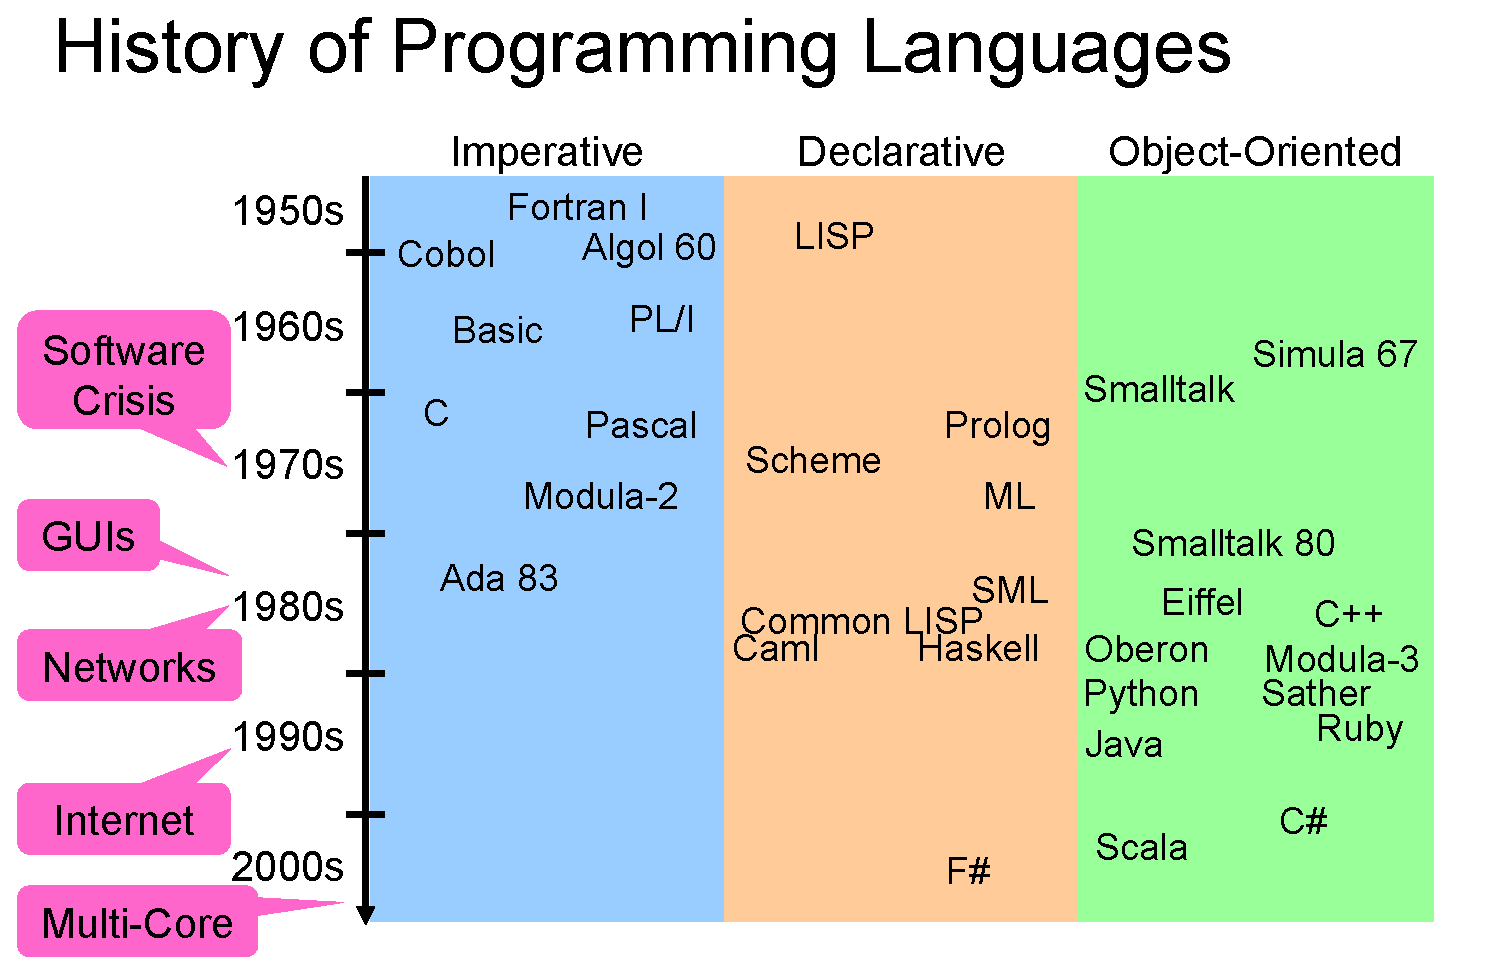
\includegraphics[width=0.7\textwidth]{img/01_programming_languages}
      \caption{History of Programming Languages}

\end{figure}

Which forced a rethinking process.
\begin{figure}[h!]
  \centering
    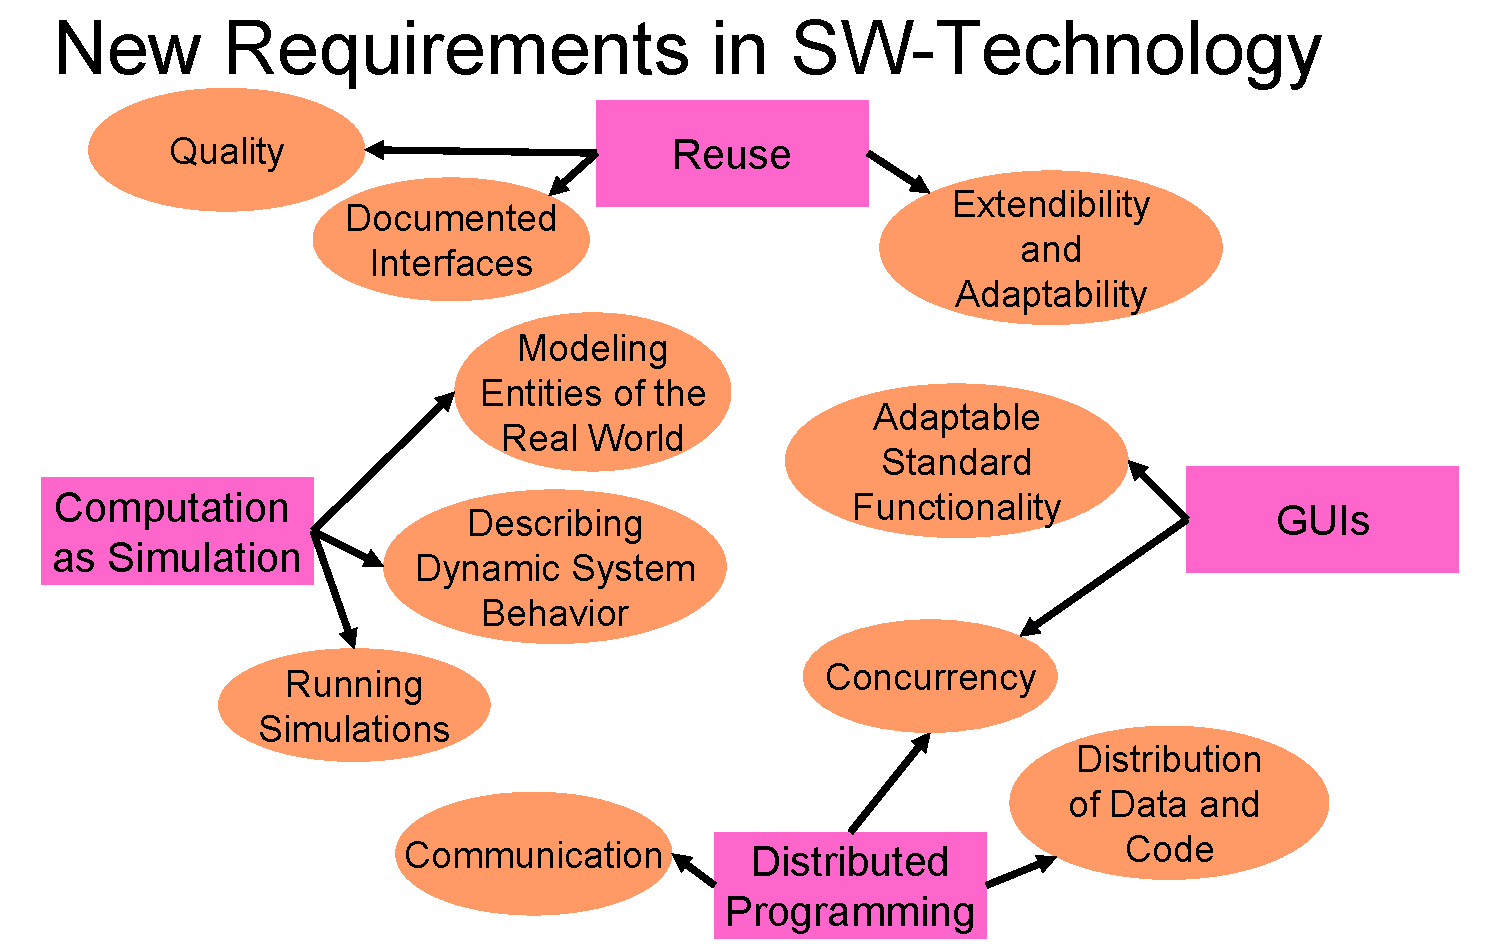
\includegraphics[width=0.7\textwidth]{img/01_new_requirements}
      \caption{New Requirements in Software Technology}
\end{figure}

\subsection{Study: Reusing Imperative Programs}
We try to model a University Administration System:
\begin{itemize}
 \item Which models students and professors
 \item Stores one record for each student and each professor in a repository
 \item A procedure printAll prints all records in the repository
\end{itemize}

\lstset{language=C}
\begin{lstlisting}[caption=Implementation in C]
typedef struct {
  char *name;
  char *room;
  char *institute;
} Professor;

typedef struct {
  char *name;
  int  regnum;
} Student;

void printStudent(Student *s) {...}
void printProf(Professor *p) {...}

typedef struct {
  enum { STU,PROF } kind;
  union {
    Student *s;
    Professor *p;
  } u;
} Person;

typedef Person **List;

void printAll(List l) {
  int i;
  for(i=0; l[ i ] != NULL; i++)
    switch(l[ i ]->kind) {
    case STU:
      printStudent(l[ i ]->u.s);
      break;
    case PROF:
      printProf(l[ i ]->u.p);
      break;
  }
}
\end{lstlisting}

\paragraph{Extending the System} in order to extend the system with assistants on has to:
\begin{itemize}
 \item Add a record and print function for the assistants
 \item Reuse old code for repository and printing
\end{itemize}

\begin{lstlisting}[caption=Extending the system]
// Student and Professor structs
typedef struct {
  char *name;
  char PhD_student; /* ‘y‘, ‘n‘ */
} Assistant;

// Student and Professor print code
void printAssi(Assistant *a) {...}

// Change the Person struct
typedef struct {
  enum { STU,PROF,ASSI } kind;
  union {
    Student *s;
    Professor *p;
    Assistant *a;
  } u;
} Person;

// Change the printAll function
void printAll(List l) {
  int i;
  for(i=0; l[ i ] != NULL; i++)
    switch(l[ i ]->kind) {
    case STU:
      printStudent(l[ i ]->u.s);
      break;
    case PROF:
      printProf(l[ i ]->u.p);
      break;
    case ASSI:
      printAssi(l[ i ]->u.a);
      break;
  }
}
\end{lstlisting}

\subsection{Reuse in Imperative Languages}
\begin{itemize}
 \item Imperative languages don't have an explicit language support for extension and adaption
 \item Adaption usually requires modification reused code
 \item Code adaption requires \textbf{Copy-and-paste reuse} which leads to
  \begin{itemize}
   \item Code duplication
   \item Is difficult to maintain
   \item Is \emph{Error-prone}
  \end{itemize}

\end{itemize}

\subsection{Core Requirements}
All of this leads to these core requirements for object oriented programming languages:
\begin{figure}[h!]
  \centering
    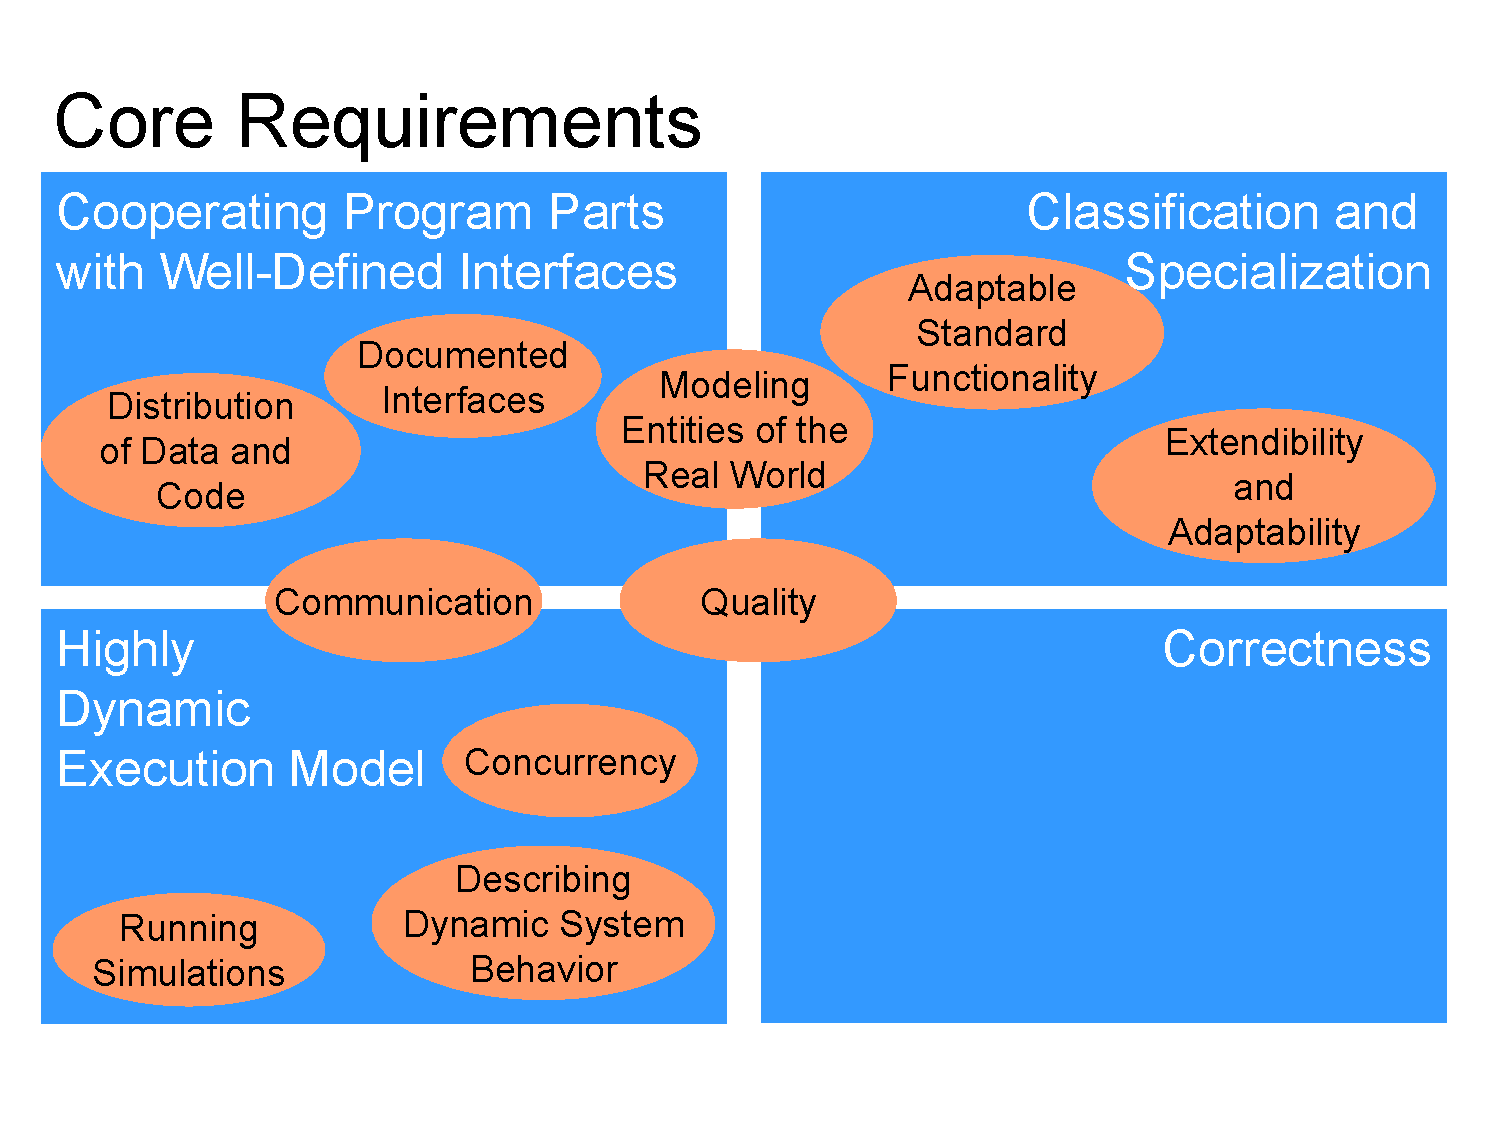
\includegraphics[width=0.7\textwidth]{img/01_core_requirements}
      \caption{Core Requirements in Software Technology}
\end{figure}

\section{Core Concepts}
\begin{shadequote}
The basic philosophy underlying object-oriented
programming is to make the programs as far as
possible reflect that part of the reality they are going
to treat. It is then often easier to understand and to
get an overview of what is described in programs.
The reason is that human beings from the outset are
used to and trained in the perception of what is going
on in the real world. The closer it is possible to use
this way of thinking in programming, the easier it is to
write and understand programs.\par\emph{Object-oriented Programming in the BETA Programming Language}
\end{shadequote}
\subsection{The Object Model}
\begin{itemize}
 \item A software system is a set of cooperating object
 \item Objects have state and processing ability
 \item Objects exchange messages
\end{itemize}
\begin{figure}[H]
  \centering
    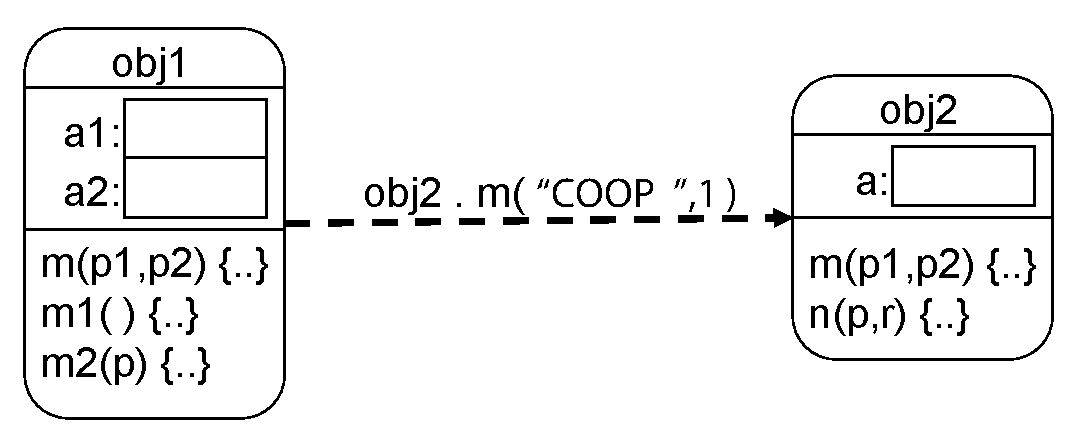
\includegraphics[width=0.5\textwidth]{img/01_object_model}
      \caption{The object model}
\end{figure}
\subsubsection{Characteristics of Objects}
\begin{itemize}
 \item State
 \item Identity
 \item Lifecycle
 \item Location
 \item Behavior
\end{itemize}
Compared to imperative programming, 
\begin{itemize}
 \item Objects lead to a \emph{different program structure}
 \item Objects lead to a \emph{different execution model}
\end{itemize}

\subsection{Interfaces and Encapsulation} 
\begin{itemize}
 \item Objects have \textbf{well-defined interfaces}
  \begin{itemize}
   \item Publicly accessible fields
   \item Publicly accessible methods
  \end{itemize}
 \item \text{Implementation is hidden} behind interface
  \begin{itemize}
   \item Encapsulation
   \item Information hiding
  \end{itemize}
 \item Interfaces are the basis for \textbf{describing behavior}
\end{itemize}

\subsection{Classification and Polymorphism}
\begin{itemize}
 \item \textbf{Classification}: Is a hierarchical structuring of objects
 \item Objects belong to different classes simultaneously
 \item \textbf{Substitution principle}: Subtype objects can be used wherever supertype objects are expected.
\end{itemize}

\begin{definition}[Classification]
Classifying is a general technique to hierarchically
structure knowledge about concepts, items, and
their properties.\\
The result is called classification.
\end{definition}

\paragraph{Characteristics of Classifications} We can classify objects or fields:
\begin{itemize}
 \item Classifications can be \emph{trees} or \emph{DAGs}
 \item Classifications of objects form \emph{``is-a'' relation}.
 \item Classes can be \emph{abstract} or \emph{concrete}.
\end{itemize}
\begin{definition}[Substitution principle]
Objects of subtypes can be used wherever objects are expected.
\end{definition}

\subsection{Polymorphism}
\begin{shadequote}
The quality of being able to assume different forms.\par\emph{Merriam-Webster Dictionary}
\end{shadequote}

\begin{definition}A program part is polymorphic if it can be used for objects of several types.
\end{definition}

\paragraph{Subtype Polymorphism} is a direct consequence of the substitution principle.
\begin{itemize}
 \item Program parts working with supertype objects work as well with subtype objects
 \item Example: \lstinline{ printAll } can print objects of class Person, Student, Professor, etc.
\end{itemize}
\subsection{Other forms of polymorphism}
\begin{description}
 \item[Parametric Polymorphism] Generic types
  \begin{itemize}
   \item Uses \emph{type parameters}
   \item One implementation can be used for different types
   \item \emph{Type mismatches can be detected at compile time}
  \end{itemize}
  \lstset{language=Java}
  \begin{lstlisting}
  class List<G> {
    G[ ] elems;
    void append(G p) { ... }
  }
  
  List<String> myList;
  myList = new List<String>();
  myList.append("String”);
  \end{lstlisting}
 \item[Ad-hoc Polymorphism] Method overloading
  \begin{itemize}
   \item Allows several methods with the \emph{same name but different arguments}
   \item Also called \emph{overloading}
   \item No semantic concept: Can be modeled by \emph{renaming}
  \end{itemize}
  \begin{lstlisting}
  class Any {
    void foo(Polar p) { ... }
    void foo(Coord c) { ... }
  }
  x.foo(new Coord(5, 10));
  x.foo(new Polar(5, 10));
  \end{lstlisting}
\end{description}

\subsection{Specialization}
\begin{definition}
 Adding specific properties to an object or refining a concept by adding further characteristics.
\end{definition}
\begin{itemize}
 \item Start from general objects or types
 \item Extend these objects and their implementations(add properties)
 \item Requirement: Behavior of specialized objects is compliant to behavior of more general objects
 \item Program parts that work for the more general objects work as well for specialized objects
 \item Implementation inheritance, reuse.
\end{itemize}

\subsection{Meeting the Requirements}
\begin{figure}[H]
  \centering
    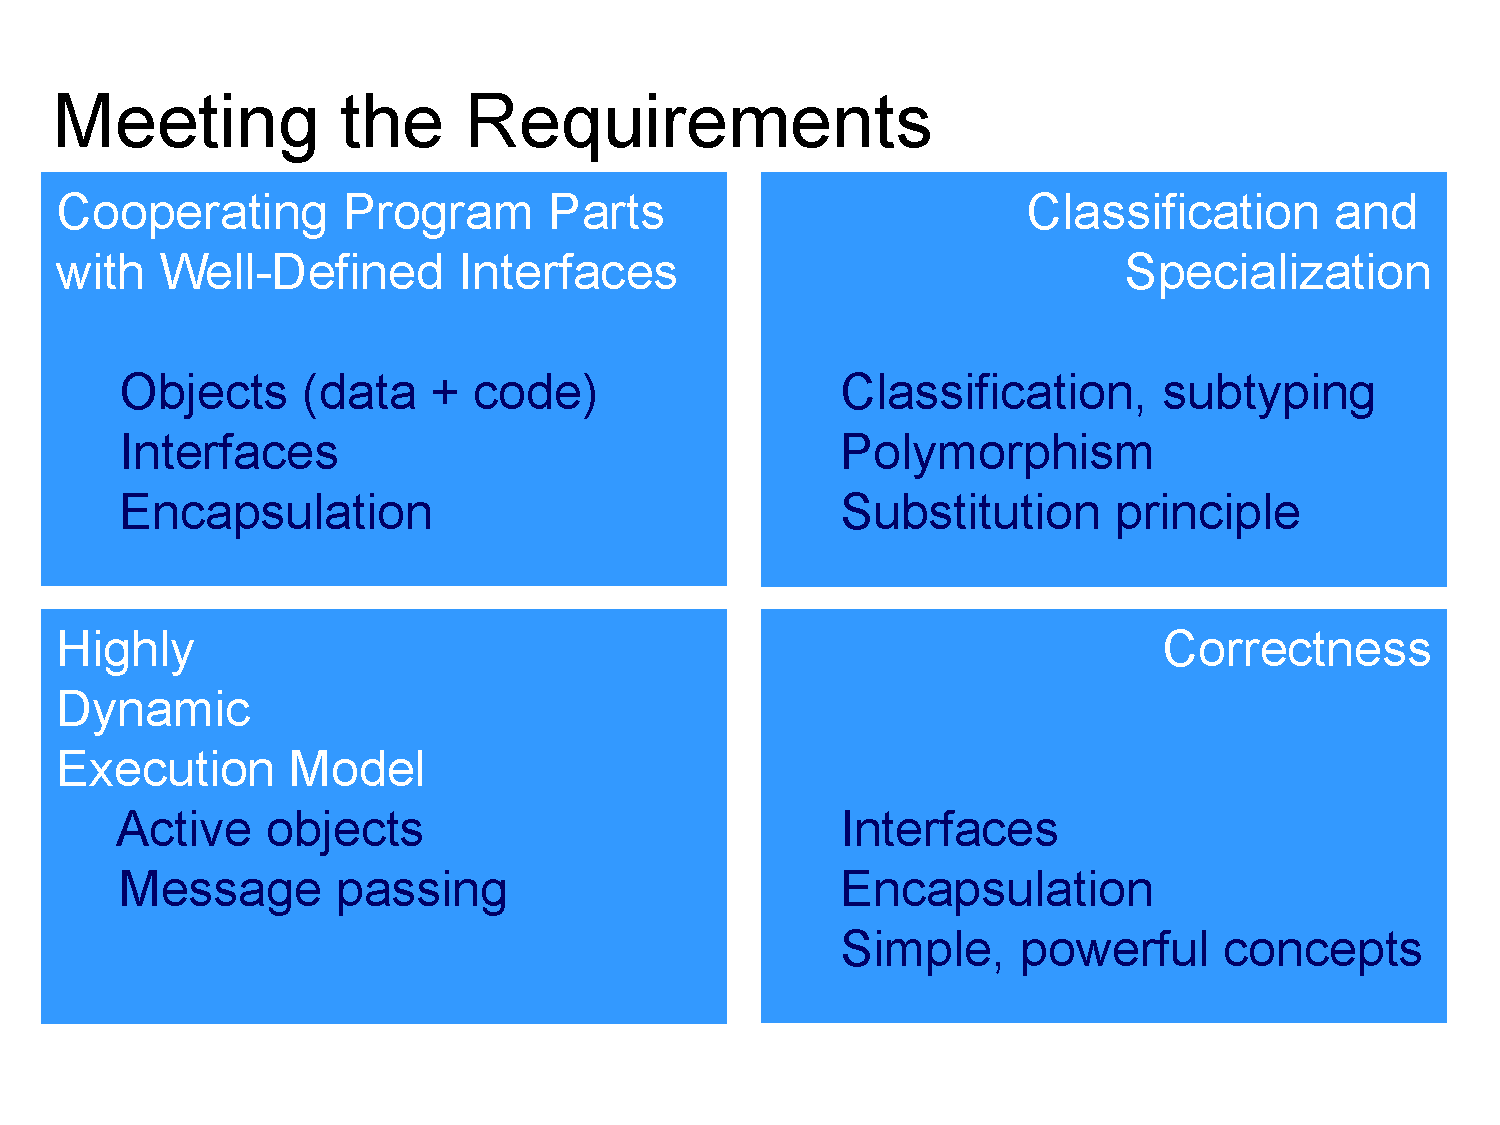
\includegraphics[width=0.7\textwidth]{img/01_meeting_the_requirements}
      \caption{Meeting the Requirements}
\end{figure}

\subsection{Summary}
Core concepts of the OO-paradigm:
\begin{itemize}
 \item Object model
 \item Interfaces and encapsulation
 \item Classification and polymorphism
\end{itemize}
Core concepts are \emph{abstract concepts} to meet the new requirements. To apply the core concepts we need ways to \emph{express them in programs}. \emph{Language concepts} enable and facilitate the application of the core concepts.


\section{Language Concepts}
% \begin{description}
%  \item[Types]
%  \item[Methods]
%  \item[Inheritance]
%  \item[Dynamic Method Binding] Method implementation is selected at runtime, depending on the type of the receiver object.
%  \begin{lstlisting}
%   void printAll(Person[ ] l) {
%     for(int i=0; l[ i ] != null; i++)
%     l[ i ] . print();
%   }
%  \end{lstlisting}
\lstset{language=C}
Why use an OO-language when we can describe a program in an imperative language?
\paragraph{Example} Previous Problem in C.
\begin{itemize}
 \item Type declaration:
 \begin{lstlisting}
  typedef char* String;
  typedef struct sPerson Person;
 \end{lstlisting}
 \item Record declaration with fields and methods (function pointers)
 \begin{lstlisting}
  struct sPerson {
    String name;
    void (*print)(Person*);
    String (*lastName)(Person*);
  };
 \end{lstlisting}
 \item Method definitions:
 \begin{lstlisting}
  void printPerson(Person *this) {
    printf("Name: %s\n", this->name);
  }
  String LN_Person(Person *this)
    {...}
 \end{lstlisting}
 \item Constructor definitions:
 \begin{lstlisting}
  Person *PersonC(String n) {
    Person *this   = (Person *) malloc(sizeof(Person));
    this->name     = n;
    this->print    = printPerson;
    this->lastName = LN_Person;
    return this;
  }
 \end{lstlisting}
 \item Using constructors, fields, and methods
 \begin{lstlisting}
  Person *p;
  p = PersonC("Tony Hoare");
  p->name = p->lastName(p);
  p->print(p);
 \end{lstlisting}
 \item Inheritance
  \begin{itemize}
   \item Copy code
   \item Adapt function signatures
   \item Define Specialized Methods
   \item Reuse Person for Student
   \item View Student as Person (cast)
  \end{itemize}
 \begin{lstlisting}
  typedef struct sStudent Student;
  struct sStudent {
    String name;
    void (*print)(Student*);
    String (*lastName)(Student*);
    int regNum;
  };
  void printStudent(Student *this) {
    printf("Name: %s\n", this->name);
    printf("No: %d\n", this->regNum);
  }
  Student *StudentC(String n, int r) {
    Student *this  = (Student *) malloc(sizeof(Student));
    this->name     = n
    this->print    = printStudent;
    this->lastName = (String (*)(Student*)) LN_Person;
    this->regNum   = r;
    return this;
  }
 \end{lstlisting}
 \item Subclassing and Dynamic Binding
  \begin{itemize}
   \item Student has all fields and methods of Person
   \item Casts are necessary
  \end{itemize}
  \begin{lstlisting}
    Student *s;
    Person *p;
    s = StudentC("Susan Roberts", 0);
    p = (Person *) s;
    p->name = p->lastName(p);
    p->print(p);
  \end{lstlisting}
  \item Methods are selected dynamically
  \begin{lstlisting}
    void printAll( Person **l ) {
      int i;
      for (i=0; l[i] != NULL; i++)
        l[i]->print(l[i]);
      }
    }
  \end{lstlisting}
\end{itemize}

\subsubsection{Discussion of the C Solution}

\paragraph{Pros} We can express \emph{objects}, \emph{fields}, \emph{methods}, \emph{constructors}, and \emph{dynamic method binding} by imitating OO-programming. The union in Person and the switch statement in \lstinline{printAll} (previous example) became dispensable.
The behavior of reused code (\lstinline{Person}, \lstinline{printAll}) can be \emph{adapted} to introduce Student \emph{without changing the implementation}.
\paragraph{Cons} Inheritance has to be replace by \emph{code duplication}. Subtyping can be simulated, but it requires:
\begin{itemize}
 \item Casts, which is \emph{not type safe}
 \item \emph{Same memory layout} of super and subclasses (same fields and function pointers in same order), which is \emph{extremely error-prone}.
\end{itemize}
Appropriate language support is needed to apply object-oriented concepts.

\subsubsection{A Java Solution}
\lstset{language=Java}
\begin{lstlisting}
class Person {
  String name;
  void print() {
    System.out.println("Name: " + name);
  }
  String lastName() {...}
  Person(String n) {name = n}
}
class Student extends Person {
  int regNum;
  void print() {
    super.print();
    System.out.println(“No: “ + regNum);
  }
  Student(String n, int i ) {
    super(n);
    regNum = i;
  }
}
void printAll(Person[] l) {
  for (int i=0; l[i] != null; i++)
    l[i].print();
}
\end{lstlisting}

The Java solution uses
\begin{description}
 \item[Inheritance] to avoid code duplication.
 \item[Subtyping] to express classification.
 \item[Overriding] to specialize methods.
 \item[Dynamic Binding] to adapt reused algorithms.
\end{description}
Java supports the OO-language concepts and the Java solution is
\begin{itemize}
 \item Simpler and smaller
 \item Easier to maintain (no duplicate code)
 \item Type safe
\end{itemize}

\subsubsection{Concepts Summary}
\begin{figure}[H]
  \centering
    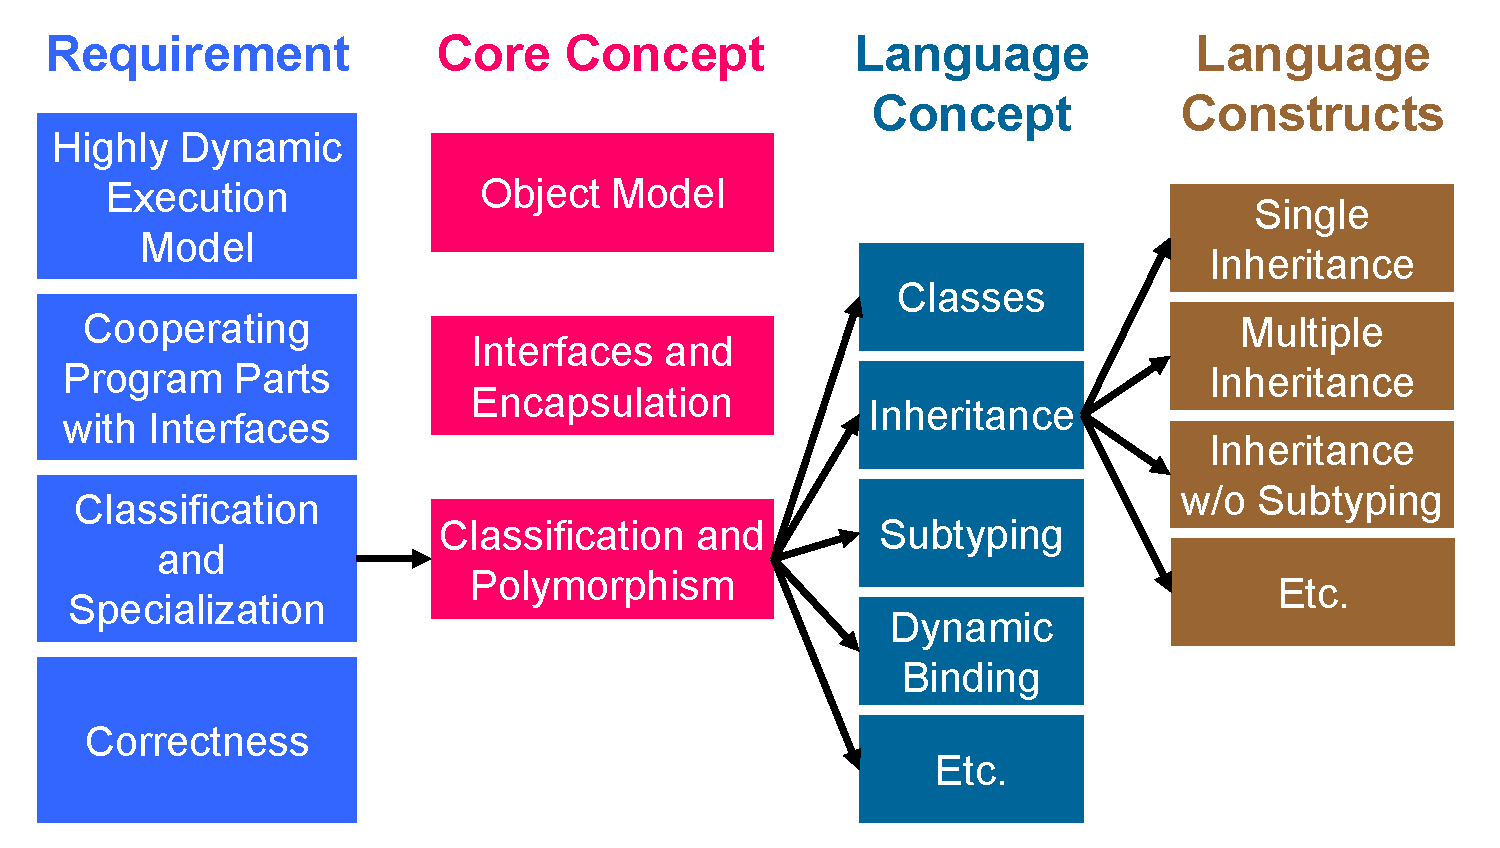
\includegraphics[width=0.7\textwidth]{img/01_concepts_summary}
      \caption{Concepts Summary}
\end{figure}

\section{Language Design}
A good language should resolve design trade-offs in a way \emph{suitable for its application domain}.
\paragraph{Design Goals} $\text{}$
\begin{description}
 \item[Simplicty] $\text{}$
  \begin{itemize}
   \item Syntax and semantics can be easily understood by users and implementers of the language.
   \item This doesn't mean that the number of constructs should be limited.
   \item Simple languages: BASIC, Pascal, C.
   \item It is not know whether the Java 5 type system (generics) is deciable.
  \end{itemize}
 \item[Expressiveness]  $\text{}$
  \begin{itemize}
   \item Language can (easily) express complex processes and structures
   \item Expressive languages: C\#, Scala, Python
   \item Expressiveness is often conflicting with simplicity:
  \end{itemize}
 \item[(Static) Safety] $\text{}$
  \begin{itemize}
   \item Language discourages errors and allows errors to be discovered and reported. Ideally at compile time.
   \item Safe languages: Java, C\#, Scala.
   \item Often conflicting with expressiveness and performance.
  \end{itemize}
 \item[Modularity]  $\text{}$
  \begin{itemize}
   \item Language allows modules to be compiled separately
   \item Modula languages: Java, C\, Scala
   \item Often conflicting with expressiveness and performance. 
  \end{itemize}
 \item[Performance]  $\text{}$
  \begin{itemize}
   \item Programs written in the language can be executed efficiently
   \item Efficient languages: C, C++, Fortran.
   \item Often conflicting with safety and productivity:
    \begin{itemize}
     \item C arrays:
      \begin{itemize}
       \item Sequence of memory locations
       \item Access is a simple look-up with only 2-5 machine instructions
      \end{itemize}
     \item Java arrays
      \begin{itemize}
       \item Sequence of memory locations \emph{plus length}
       \item Access is look-up \emph{plus bound-check}
      \end{itemize}
    \end{itemize}
  \end{itemize}
 \item[Productivity]  $\text{}$
  \begin{itemize}
   \item Language leads to low costs of writing programs
   \item Closely related to expressiveness
   \item Languages for high productivity:
    \begin{itemize}
     \item Visual Basic
     \item Python
    \end{itemize}
   \item Often conflicting with static safety
  \end{itemize}
 \item[Backwards Compatibility]  $\text{}$
  \begin{itemize}
   \item Newer language version work and interface with programs in older version
   \item Backwards compatible languages:
    \begin{itemize}
     \item Java
      \begin{lstlisting}
      class Tuple<T> {
        T first; T second;
        void set(T first, T second) {
          this.first = first;
          this.second = second;
        }
      }
      class Client {
        static void main(String[] args) {
          Tuple t = new Tuple();
          t.set("Hello", new Client());
        }
      }
      \end{lstlisting}

     \item C
    \end{itemize}
   \item Often in conflict with simplicity and performance.
  \end{itemize}


\end{description}
